\section{Tömítés kiválasztása}

\begin{figure}[hbt!]
	\centering
	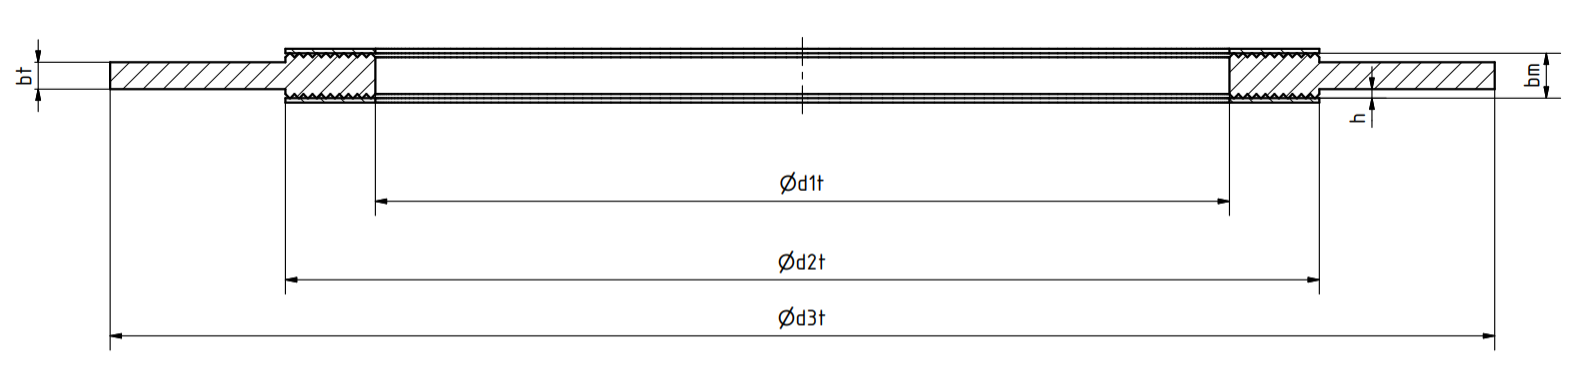
\includegraphics[scale=.34]{./images/tomites.png}
	\caption{Tömítés előtervének rajza}
\end{figure}
\begin{align*}
	&d_1 = \siunit{\tomdone}{\mm} \\
	&d_2 = \siunit{\tomdtwo}{\mm} \\
	&d_3 = \siunit{\tomdthree}{\mm} \\
	&b_t = \siunit{\tombt}{\mm} \\
	&b_m = \siunit{\tombm}{\mm} \\
	&h_{\text{max}} = \siunit{\tomhmax}{\mm} \\
	&h_{\text{min}} = \siunit{\tomhmin}{\mm}
\end{align*}
